\chapter{Моделирование TGE и TGF
}\label{ch:thunderstorm}

\section{Обзор экспериментальных результатов
}\label{sec:thunderstorm/review-exp}

\section{Обзор существующих моделей}\label{sec:thunderstorm/review-mod}

\subsection{Пробой на убегающих электронах}
%
Пробой на убегающих электронах (ПУЭ) --- модель развития лавины релятивистских (с энергией 0.1 --- 10 МэВ) электронов в постоянном электрическом поле предложенная А.~В.~Гуревичем~\cite{gurevich1992runaway,Gurevich2001ufn}. Качественно идея модели проста: пусть электрон ускоряется за счет электрического поля и тормозится за счет взаимодействия со средой, если он получает от поля больше энергии чем теряет, то у него появляется избыток энергии, который может быть потрачен на рождение нового электрона. Такие электроны будем называть убегающими. Если пренебречь всеми процессами кроме ионизационных потерь и радиационных потерь, то \todo{график} показывает условия генерации лавины убегающих электронов в однородном поле. Энергию при которой электрон в среднем на единице длинны приобретает энергии больше чем теряет мы будем называть критической.

\subsection{Модели атмосферы}
Для устанаволения значения плотности воздуха на разных высотах в моделировании используется международная стандартная модель атмосферы (ISA)


\section{Моделирование RREA, сравнение с результатами Гуревича, Орешкина.}\label{sec:thunderstorm/rrea}



\section{Расчет коэффициента обратной связи, сравнение с результатами Дваера}\label{sec:thunderstorm/rdfm}
\section{Reactor like TGE-model}\label{sec:thunderstorm/reactor}

\begin{figure}[t]
    \begin{center}
        \begin{minipage}[h]{0.49\linewidth}
            \center{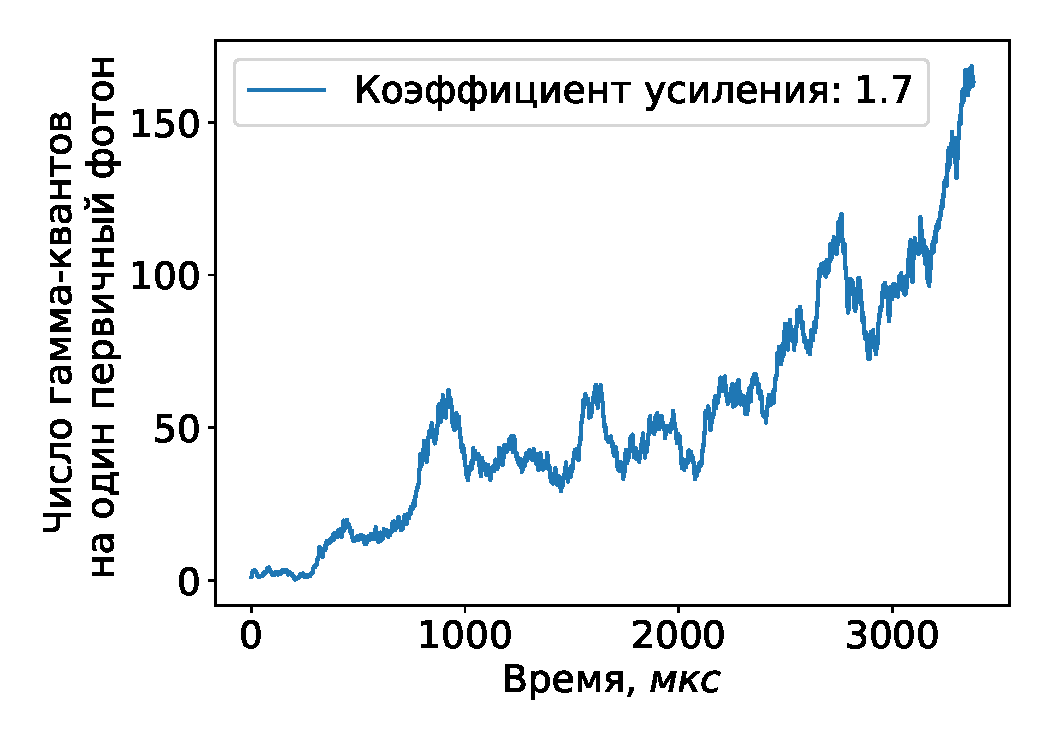
\includegraphics[width=\linewidth]{thunderstorm/RL_proofTGE.pdf} \\ а)}
        \end{minipage}
        \hfill
        \begin{minipage}[h]{0.49\linewidth}
            \center{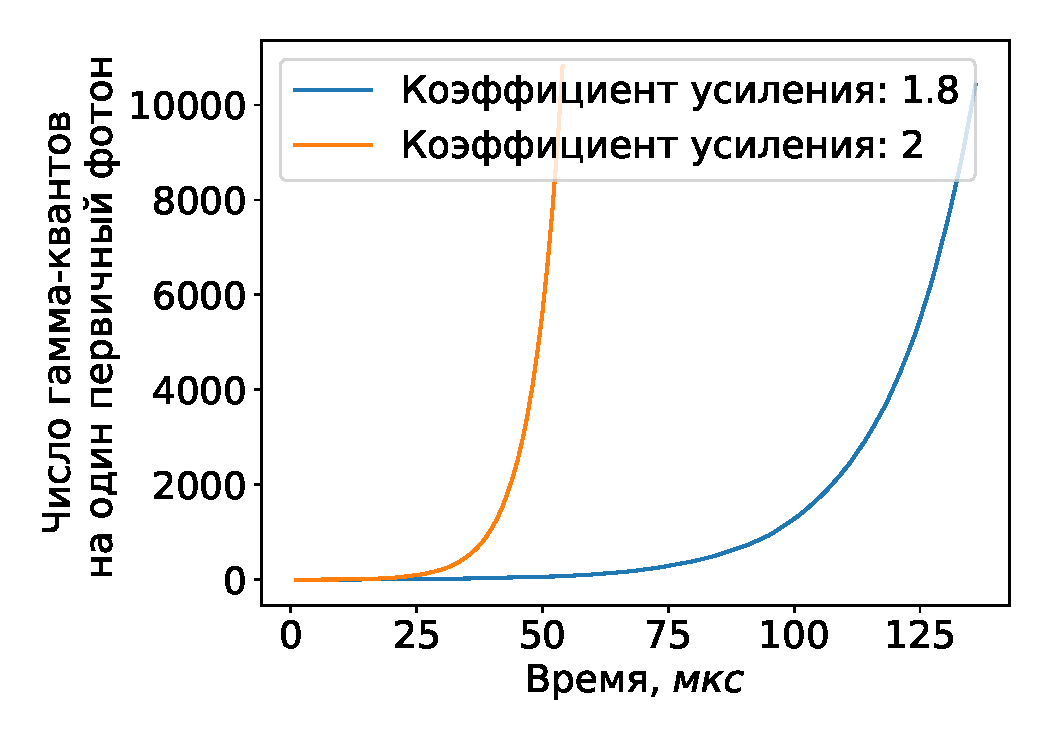
\includegraphics[width=\linewidth]{thunderstorm/RL_proofTGF.pdf}   \\ б)}
        \end{minipage}
        \caption{а) TGE-подобное нарастание. б) TGF-подобное нарастание.}
    \end{center}
    \label{thunder:rl_1}
\end{figure}


\begin{figure}[t]
    \begin{center}
        \begin{minipage}[h]{0.49\linewidth}
            \center{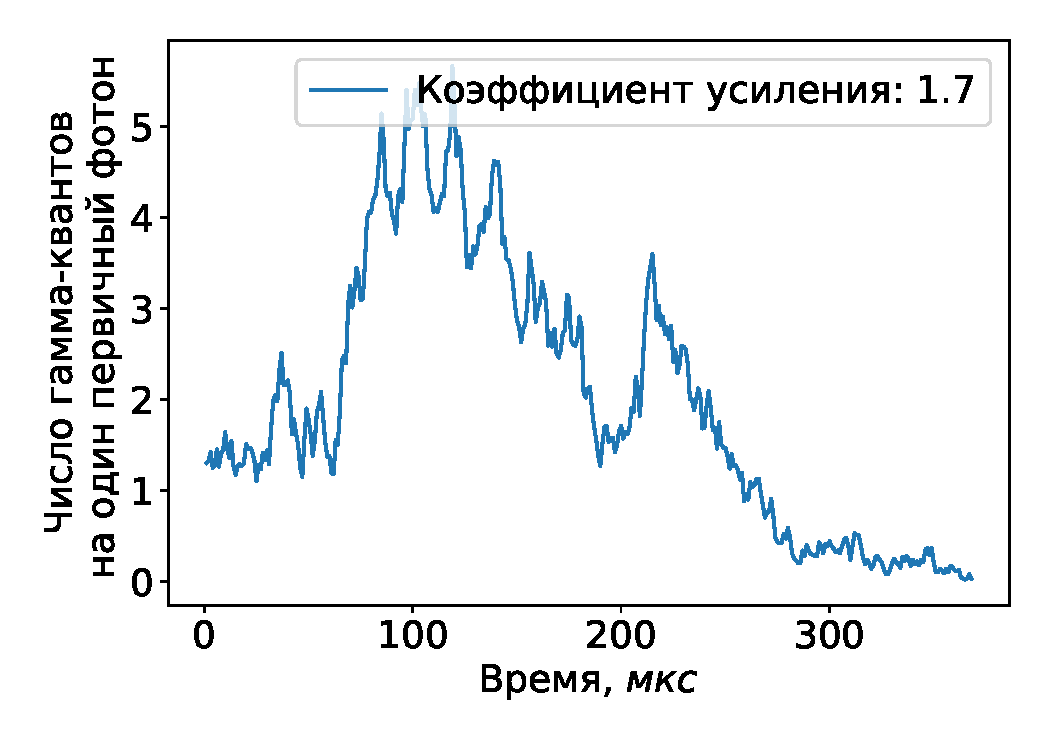
\includegraphics[width=\linewidth]{thunderstorm/RL_Extinction.pdf} \\ а)}
        \end{minipage}
        \hfill
        \begin{minipage}[h]{0.49\linewidth}
            \center{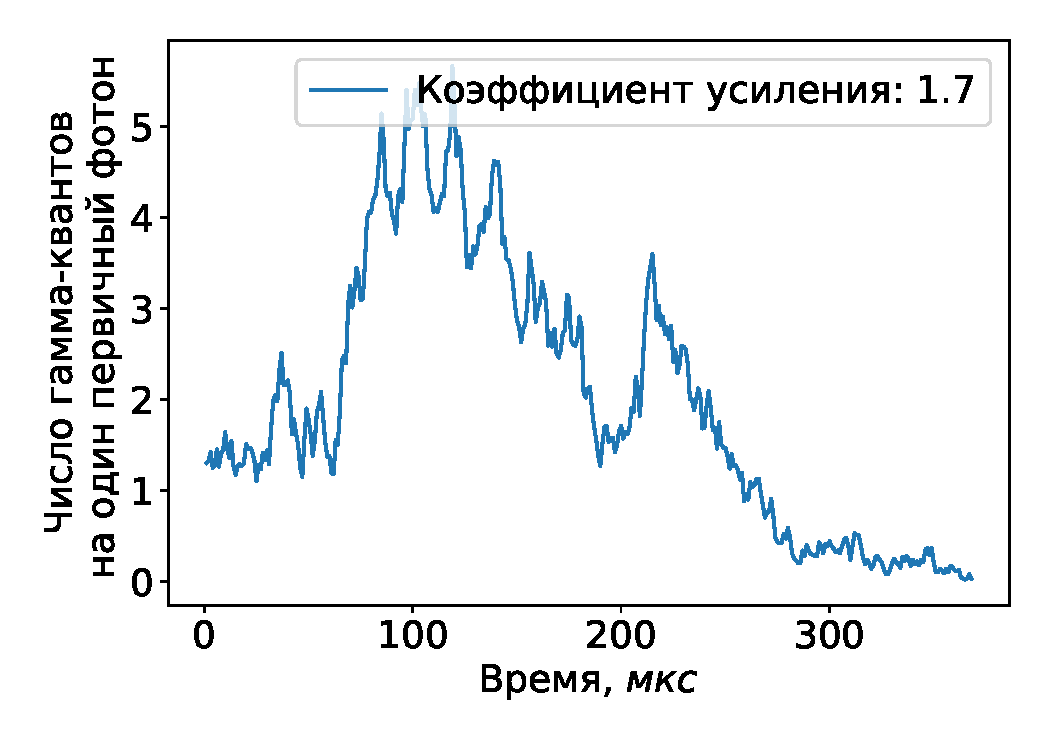
\includegraphics[width=\linewidth]{thunderstorm/RL_Extinction.pdf}   \\ б)}
        \end{minipage}
        \caption{а) Затухание лавины. б) placeholder.}
    \end{center}
    \label{thunder:rl_2}
\end{figure}

\clearpage